
% Revisado por Cristina el día 12/03/2013

\srsfuncion{Consultar inventario} \label{fun:ConsulInv}
	Esta función muestra al usuario la lista completa de los items del inventario de la empresa.
		
	\begin{enumerate}
		\item \textit{Prioridad}: alta.
		\item \textit{Entradas}
		\begin{enumerate}
			\item Los items del inventario se muestran ordenados por defecto por orden alfabético, pero pueden ordenarse de acuerdo a diversos campos (fecha de entrada en almacén, cantidad de items, destino de uso (oficina, mecánica, edificios, aeronáutico\ldots) y valor de adquisición).
		\end{enumerate}
		\item \textit{Flujo de operaciones}
		\begin{enumerate}
			\item Se muestra por pantalla la lista de items disponibles en el inventario ordenada por orden alfabético. Se da la opción al usuario de ordenarla siguiendo los criterios anteriormente mencionados, cada uno de los cuales aparece en la parte superior de la tabla.
		\end{enumerate}
		\item \textit{Respuesta a situaciones no previstas}
		\begin{enumerate}
			\item Si no se puede acceder a la base de datos del inventario, se muestra por pantalla un mensaje de error y se vuelve al menú principal del sistema.
		\end{enumerate}
	\end{enumerate}
	
\begin{figure}[ht]\centering
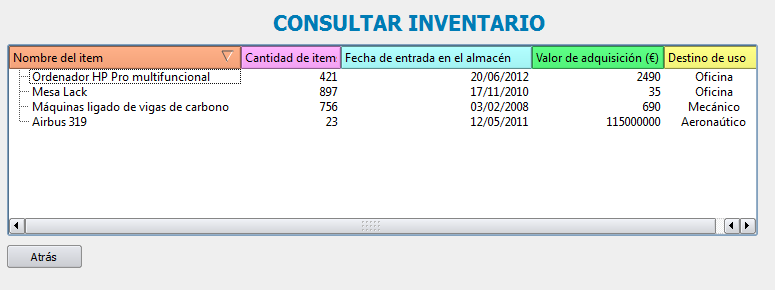
\includegraphics[scale=.6]{imagenes/consultarInventarioImagen.png}
\caption{Pantalla aproximada de la consulta de inventario}
\end{figure}